\documentclass[11pt]{article}

% Informations

% Modules 
\usepackage[greek,english]{babel}
\usepackage{graphicx}                       % Gestion des images
\usepackage{caption}                        % Gestion des titres
\usepackage{appendix}                       % Gestion de l'annexe
\usepackage[utf8]{inputenc}                 % Encodage du texte
\usepackage{multicol}                       % Gestion des multi-colonnes des tableaux
\usepackage{booktabs}                       % Importation des traits horizontaux des tableaux
\usepackage{siunitx}                        % Gestion des unités
\usepackage{mwe,lipsum}                     % Modules de Minimal Working Examples
\usepackage{amsmath,amssymb,amsbsy}         % Ajout d'options dans le mode 'math'
\usepackage{todonotes}                      % Ajout des notes en marge
\usepackage{mathtools}                      % Autres outils pour le mode 'math'
\usepackage{hyperref}            % Gestion des hyper-liens (internes et url)
\usepackage[a4paper]{geometry}                       % Options de mise en page
\usepackage{listings}
\usepackage{color,xcolor}
\usepackage{csquotes}
\usepackage{textcomp}
\usepackage{fancyhdr}
\usepackage[T1]{fontenc}
\usepackage{lato}
\usepackage{titling}
\usepackage{datetime}
\usepackage[version=4]{mhchem}
\usepackage{authblk}
\usepackage{enumitem}
\usepackage{tablefootnote}
\usepackage{cases}
\usepackage{bbm}
\usepackage{lmodern}


\setitemize{itemsep=0pt}

% Police d'écriture
\renewcommand\familydefault{\sfdefault}

% Définition de couleurs
% \definecolor{Bleu_ENSPS}{RGB}{0,119,139}
\definecolor{CIRED_blue}{RGB}{6,100,110}
\hypersetup{
    hidelinks,
    }

% Options de biliographie 
\usepackage[style=authoryear,giveninits=true,sorting=nty,maxcitenames=1]{biblatex}
% \usepackage[backend=biber, bibstyle=ieee, citestyle=numeric-comp,
%   sorting=none, labeldateparts,
%   maxbibnames=99, maxcitenames=2, mincitenames=1]{biblatex} 
\DefineBibliographyExtras{french}{\restorecommand\mkbibnamefamily}

\AtEveryBibitem{%
  \clearlist{language}%
  \clearlist{urldate}
  \clearlist{url}
  \clearfield{month}
  \clearfield{day}
  \clearfield{note}
}
\DeclareFieldFormat{url}{}
\DeclareFieldFormat{urldate}{}

\DeclareFieldFormat{journaltitle}{\textit{#1}}
\DeclareFieldFormat{title}{#1}

\setlength\bibitemsep{\itemsep}
\AtEveryCite{\color{CIRED_blue}}

\addbibresource{/home/amounier/Documents/Bibliographie/bibliographie_bib.bib}
\bibliography{biblatex-examples.bib}

% All name in hyperlink (cite biblatex)
\makeatletter
\let\abx@macro@citeOrig\abx@macro@cite
\renewbibmacro{cite}{%
   \bibhyperref{%
   \let\bibhyperref\relax\relax%
   \abx@macro@citeOrig%
   }%
}
\let\abx@macro@textciteOrig\abx@macro@textcite
\renewbibmacro{textcite}{%
   \bibhyperref{%
   \let\bibhyperref\relax\relax%
   \abx@macro@textciteOrig%
   }%
}%
\makeatother

% Options de format pour les unités (SIUnitX package)
\sisetup{
    detect-all,
    locale                  = UK,
    sticky-per,
    inter-unit-product      = {.},
    per-mode                = reciprocal-positive-first,
}

\DeclareSIUnit\octet{o}
\DeclareSIUnit\watthour{Wh}
\DeclareSIUnit\year{yr}
\DeclareSIUnit\hab{inhab}

%Options de largeur de marges, verticales et horizontales
\geometry{hmargin=3cm,vmargin=2cm}
\setlength{\parindent}{7mm}

% Mise en page
% \pagestyle{fancy}
% \setlength{\headheight}{14pt}
% \renewcommand\headrulewidth{0.5pt}
% \renewcommand\footrulewidth{0.5pt}
% \fancyhead[C]{\thedate}
% \fancyhead[R]{}
% \fancyhead[L]{}
% \fancyhead[R]{\rightmark}

% Styles équations
%\numberwithin{equation}{section}

\makeatletter
\renewcommand\p@figure{Figure~\@ }
\makeatother

\makeatletter
\renewcommand\p@table{Table~\@ }
\makeatother

%Autres commandes
\addto\captionsfrench{
  \renewcommand{\contentsname}%
    {Sommaire}%
}

% Keywords command
\providecommand{\keywords}[1]
{
  \small    
  \textbf{\textit{Keywords~--}} #1
}

% Titre ---------------------------------------
\date{\today}
\title{Interactions between summer and winter thermal comfort, effects of climate change on optimal renovation actions}

\author[1,3,4]{André Mounier}
\author[2,3]{Louis-Gaëtan Giraudet}
\author[4]{Philippe Drobinski}
\affil[1]{\small{Agence de l'environnement et de la maîtrise de l'énergie (ADEME), Angers, France}}
\affil[2]{\small{ENPC - Institut Polytechnique de Paris, Champs-sur-Marne, France}}
\affil[3]{\small{CIRED -- ENPC, AgroParisTech, EHESS, Cirad, CNRS, Nogent-sur-Marne, France}}
\affil[4]{\small{LMD -- IPSL, École Polytechnique - IPP, ENS - PSL , Sorbonne Université, CNRS, Palaiseau, France}}

\begin{document}


\maketitle

% Contenu -------------------------------------

% Méthode :
% https://www.nature.com/documents/nature-summary-paragraph.pdf
\begin{abstract}
    Energy efficiency building renovation, particularly through thermal insulation, is a key factor in the transformation of the building stock to reduce greenhouse gas emissions and adapt dwellings to future climates. Thermal renovation of buildings is a particularly costly operation that rarely pays off for the person carrying out the work. In France, many renovation projects are financed in part by the state, and this funding involves targeting the most effective works. However, this efficiency is only measured in terms of heating needs, while the critical nature of the inadequacy of housing for future heat increases year on year.  Taking account of climate change, its future evolution, and the need to adapt homes will therefore influence the optimum renovations to target as a priority now. Here we show that the displacement of the optimum differs according to the type of building and the intensity of warming, and according to the type of renovation work. This study presents a first way of considering dynamic, energy and economic optimisations, with RC modelling of building typologies. The conclusions are different depending on the type of action carried out: for example, the insulation of opaque walls does have an antagonistic effect on heating and cooling needs (but this is particularly visible in the coldest meteorological years and without night-time natural over-ventilation), but total energy needs are always decreasing. Thus, inter-annual variations in typology and weather play a decisive role in defining the optimum. The results call into question the selection criteria for subsidised renovations, as well as the renovations carried out in practice in France. The question of the interaction between summer and winter comfort has been raised in official reports in France, because adaptation is underdeveloped, and the majority of measures are focused on winter thermal comfort. We could ask the following (deliberately provocative) question: ‘Do we need to renovate buildings on a massive scale if the French climate warms up significantly between now and the end of the century? The answer is yes, but not for all buildings or all regions in the same way. 
\end{abstract}

\keywords{Thermal insulation, Heating and cooling needs, Adaptation, Mitigation}

\clearpage
\tableofcontents

\clearpage

\section{Introduction}
\label{sec:intro}


\section{RC analogy modelling}
\label{sec:rc}

    \subsection{RC analogy and computation} % (fold)
    \label{sub:rc_analogy_and_computation}

        \subsubsection{RC analogy} % (fold)
        \label{ssub:rc_analogy}
        
        % subsubsection rc_analogy (end)

        \subsubsection{Model construction} % (fold)
        \label{ssub:model_construction}
        
        % subsubsection model_construction (end)

        \subsubsection{Model computation} % (fold)
        \label{ssub:model_computation}
        
        % subsubsection model_computation (end)

    % subsection rc_analogy_and_computation (end)

    \subsection{TABULA typologies} % (fold)
    \label{sub:tabula_typologies}
    
    (\cite{loga_tabula_2016})

    % subsection tabula_typologies (end)

    \subsection{Weather data} % (fold)
    \label{sub:weather_data}

        \subsubsection{French climate zones} % (fold)
        \label{ssub:french_climate_zones}

        
        \begin{figure}[ht]
            \centering
            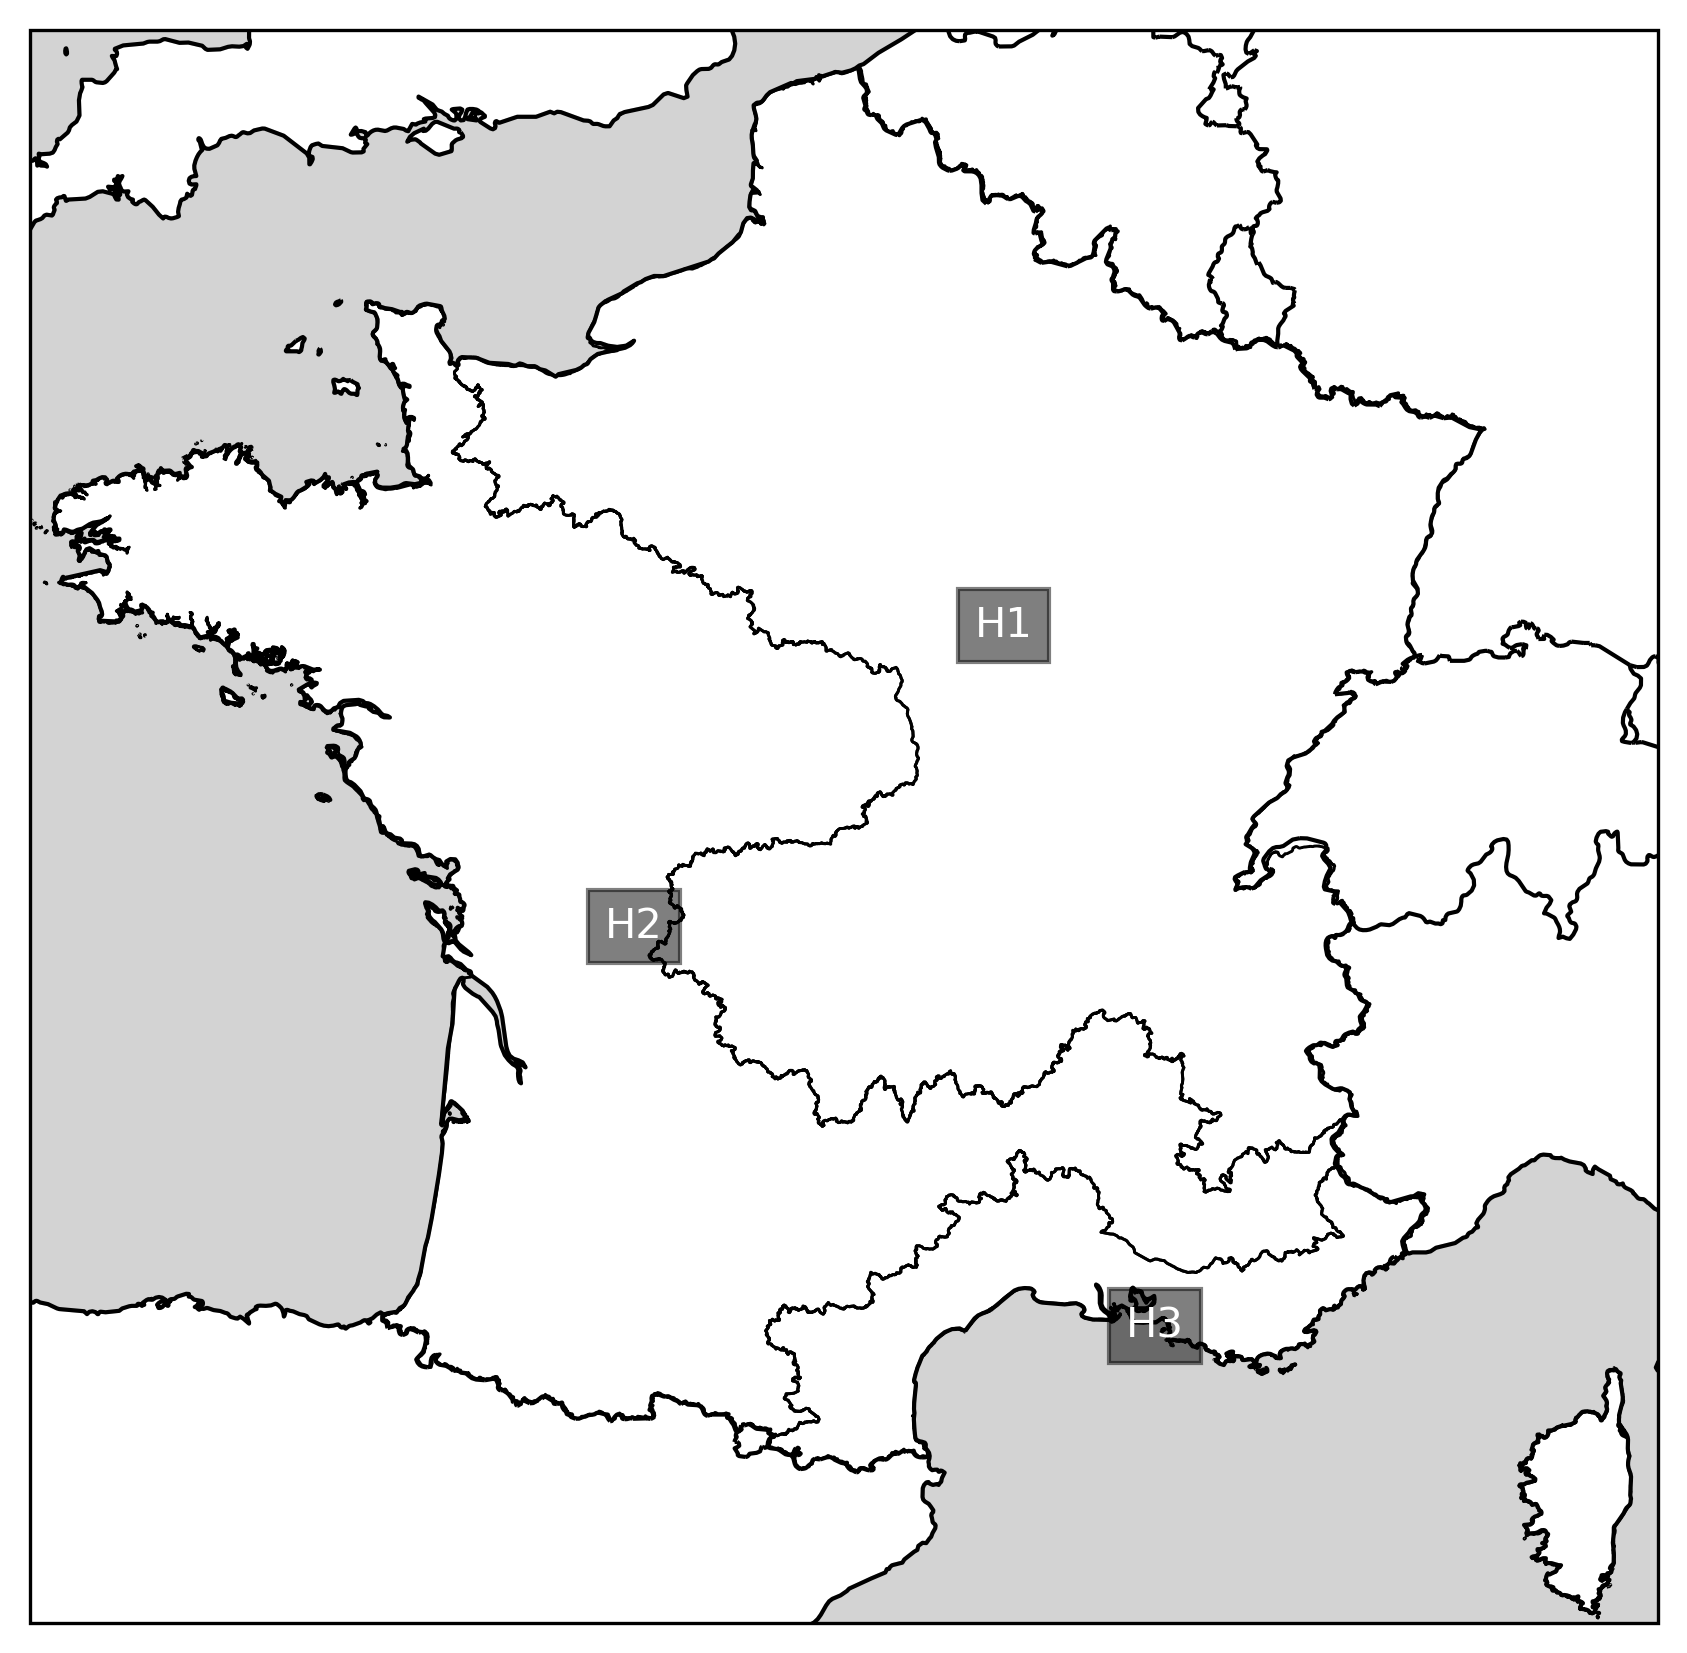
\includegraphics[width=0.32\columnwidth]{figures/zcl_winter.png}
            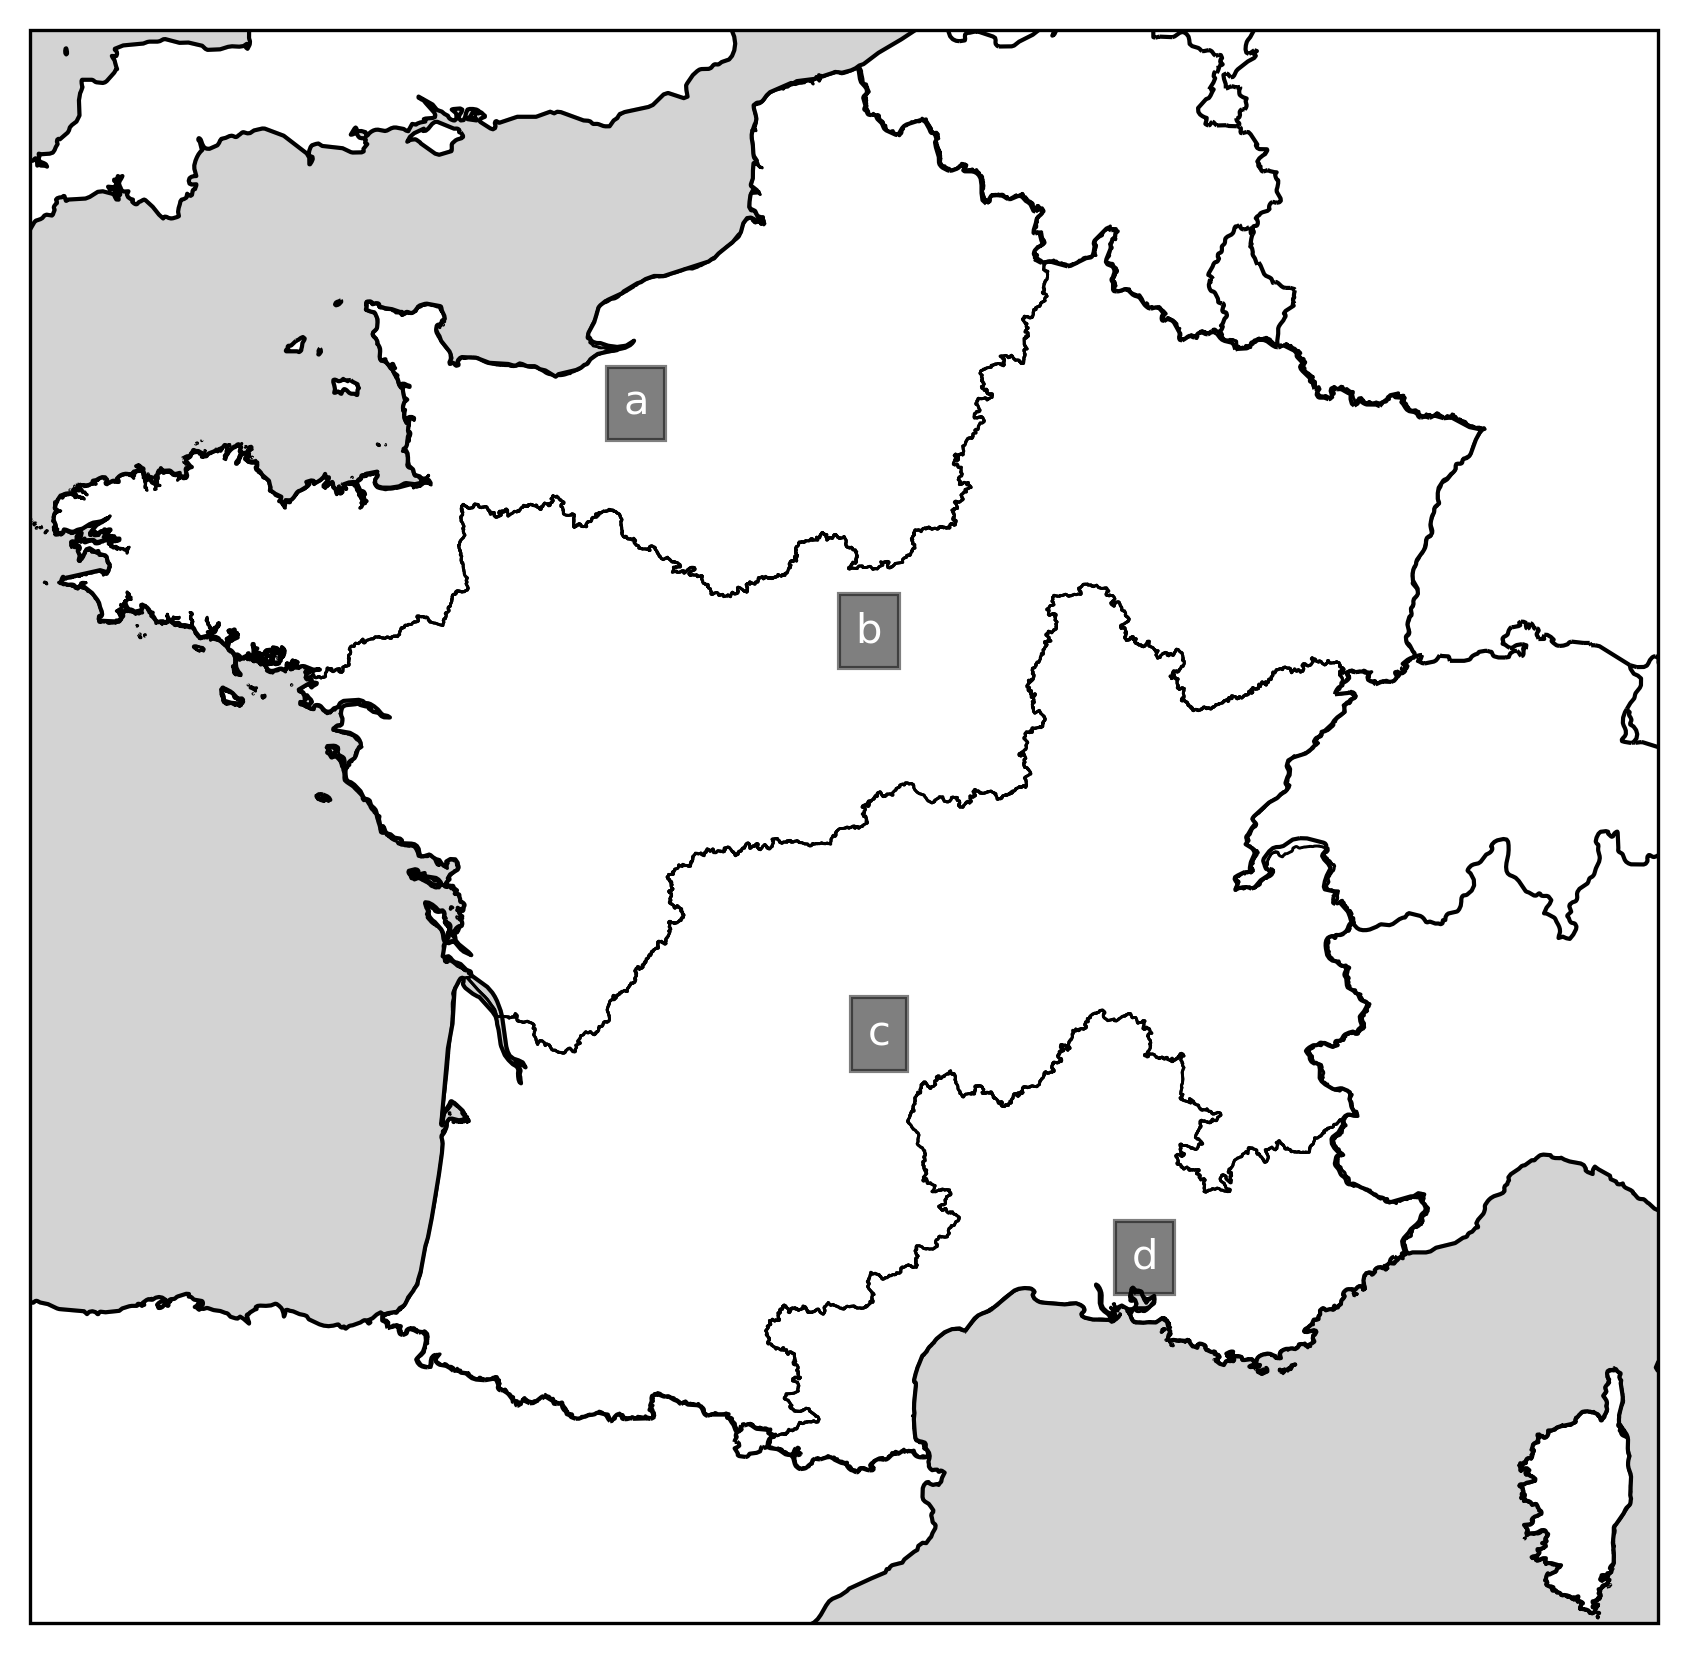
\includegraphics[width=0.32\columnwidth]{figures/zcl_summer.png}
            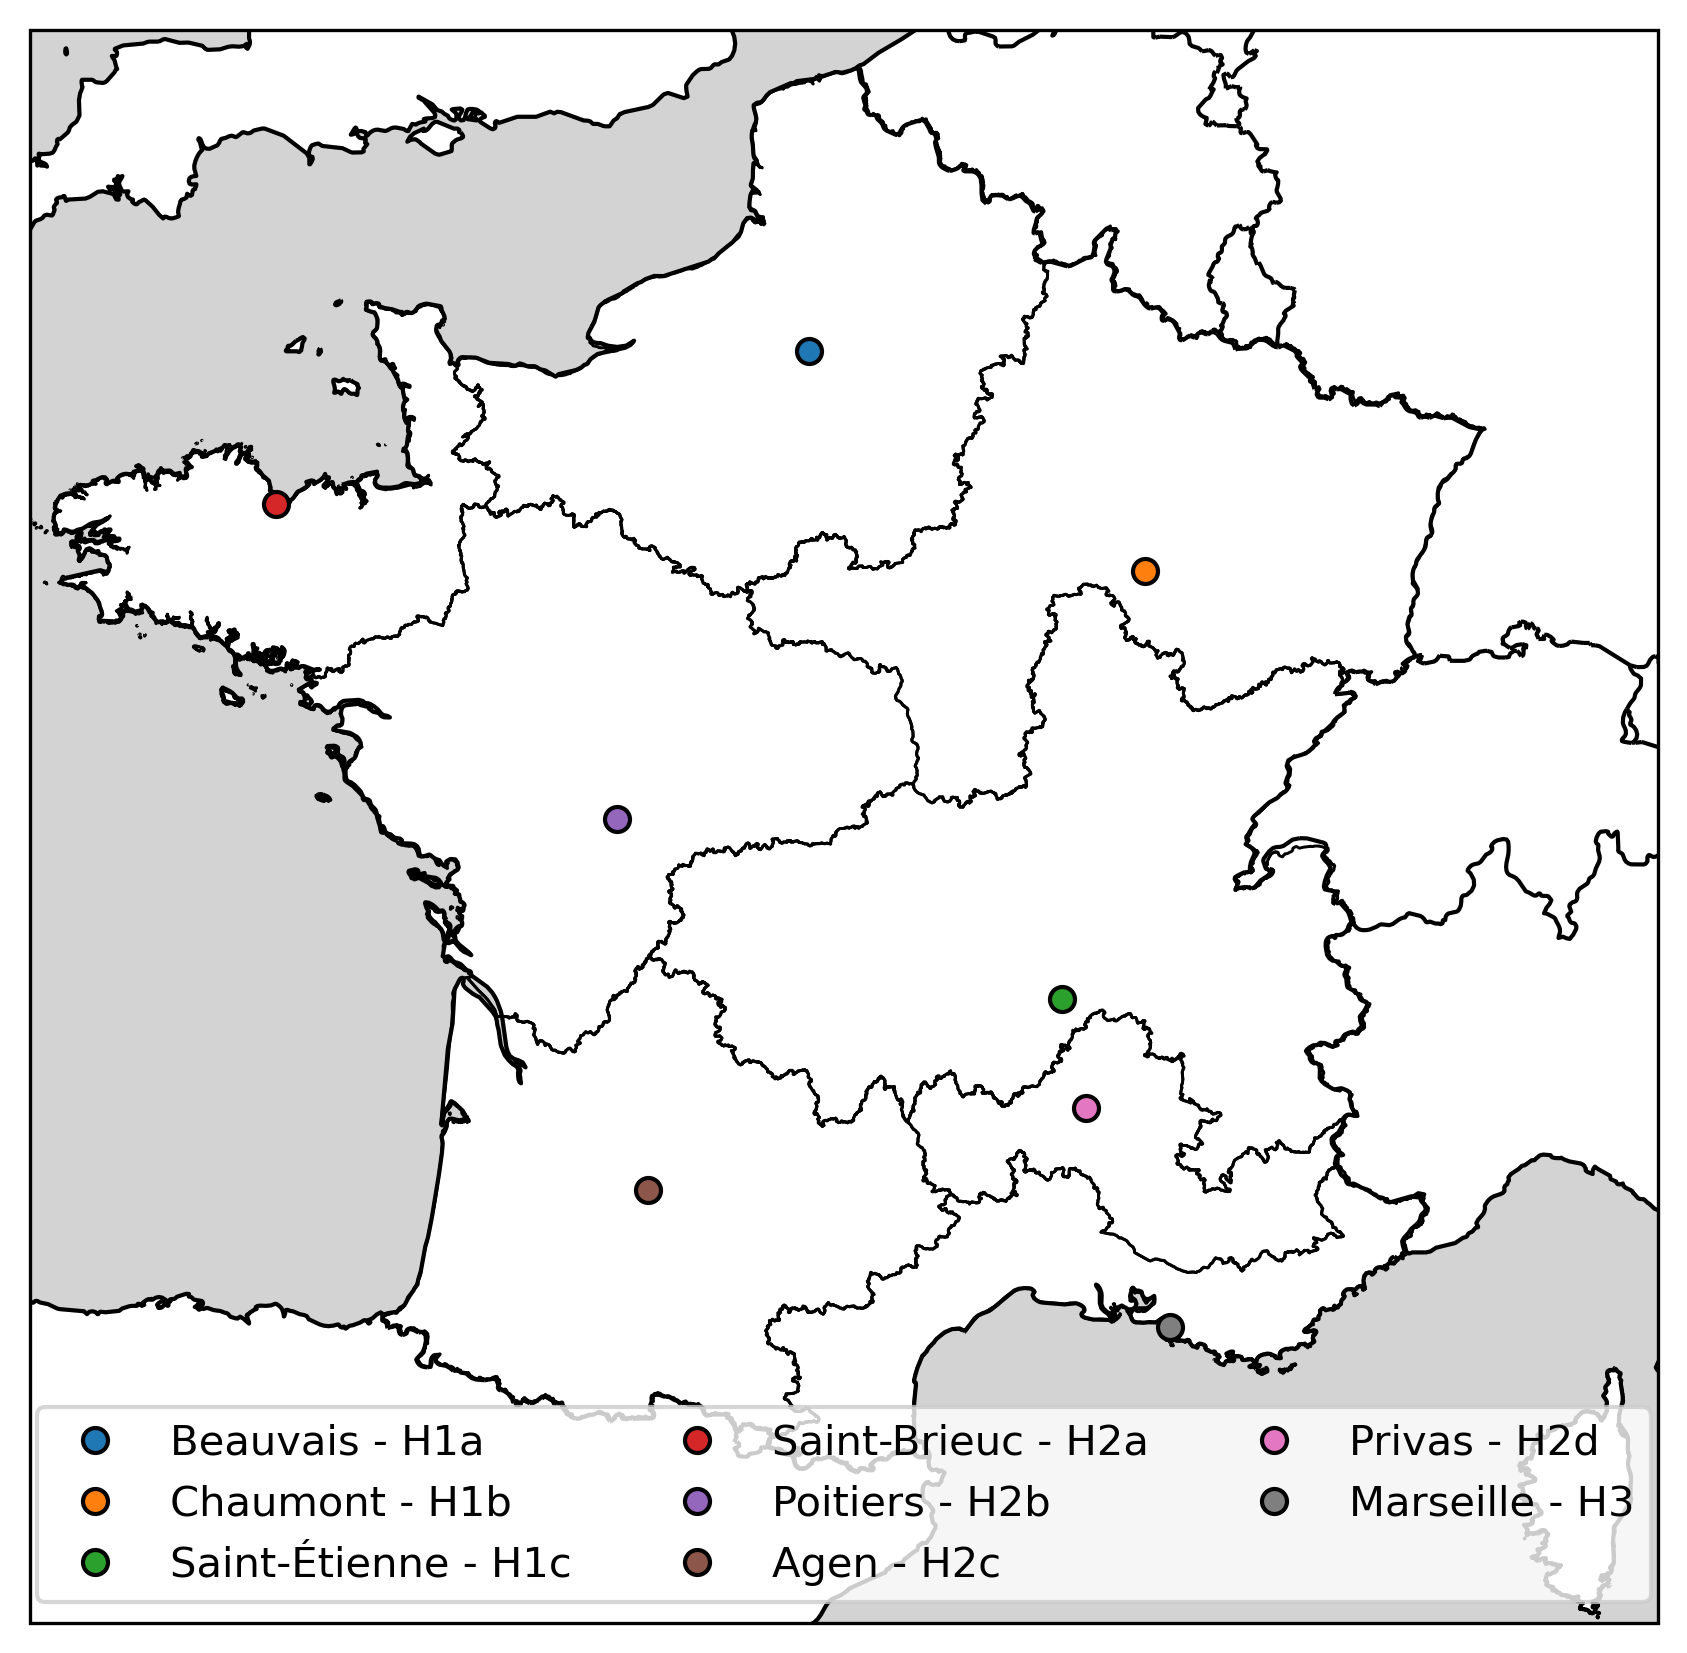
\includegraphics[width=0.32\columnwidth]{figures/zcl.png}
            \caption{\label{fig:zcl} Maps of french climate zones.}
            \begin{quote}
                \vspace{-2mm}
                \small\noindent
                \textbf{(left to right)} Map of \enquote{winter}, \enquote{summer} and combined climate zones. The winter climate zones were defined in a 1988 decree on the thermal characteristics of residential buildings (\cite{jorf_arrete_1988}). Corsica is part of region H3. Summer climate zones were defined in 2000 in parallel with new thermal regulation laws (\cite{jorf_arrete_2000}). The 8 climate zones are a combination of the two zone types (\cite{jorf_arrete_2012}) and the map shows the \enquote{central prefectures} used to define the meteorological data for each zone. 
                
                 
              \end{quote}
        \end{figure}
        
        % subsubsection french_climate_zones (end)
        \subsubsection{Historical data} % (fold)
        \label{ssub:historical_data}
        
        % subsubsection historical_data (end)

        \subsubsection{Projection data} % (fold)
        \label{ssub:projection_data}
        
        % subsubsection projection_data (end)

        \subsubsection{Standard weather data} % (fold)
        \label{ssub:standard_weather_data}
        
        % subsubsection standard_weather_data (end)
    
    % subsection weather_data (end)

    \subsection{Behaviour definition} % (fold)
    \label{sub:behaviour_definition}


    
    % subsection behaviour_definition (end)
% section rc (end)


\section{Interactions between summer and winter comfort}
\label{sec:inter}

    \subsection{Characterisation of single renovation actions} % (fold)
        \label{sub:characterisation_of_single_renovation_actions}
        
        % subsection characterisation_of_single_renovation_actions (end)    

    \subsection{Energy needs for TABULA typologies} % (fold)
    \label{sub:energy_needs_for_tabula_typologies}
    
    % subsection energy_needs_for_tabula_typologies (end)
% section inter (end)

\section{Climate impact on optimal renovations}
\label{sec:opti}

    \subsection{Optimal energy efficiency} % (fold)
    \label{sub:optimal_energy_efficiency}
    
    % subsection optimal_energy_efficiency (end)

    \subsection{Optimal economic efficiency} % (fold)
    \label{sub:optimal_economic_efficiency}
    
    % subsection optimal_economic_efficiency (end)
% section opti (end)

% \section{Generalisation across the entire french building stock}
% \label{sec:generalisation}

% % section generalisation (end)

\section{Discussion}
\label{sec:disc}
% section disc (end)

\section{Conclusion}
\label{sec:conclu}
% section conclu (end)



\clearpage
\printbibliography


\end{document}